%!TEX root = ../thesis.tex
% This paragraph covered a lot of ground, but I was a bit lost since each sentence tried to cover too many different approaches. Is there an implied structure? E.g. first software-static, then software-video, then physical tasks? Id’ have expected some more basic references early on that for example show that people don’t read software documentation and instead look for task-centered learning materials. There’s also a difference between related work that investigates what good instruction formats are, and systems work that introduces new tools to create such formats.

\chapter{Background}
\label{chapter_background}

This dissertation proposes computational methods to create interactive tutorials for software applications and physical tasks. To ground our work in existing practices and principles, in this chapter, I define the terminology commonly used by tutorial researchers and online communities (Section \ref{background_terms}).
%
I survey research studies and literature about the motivations of people creating, sharing, and consuming tutorials (Section \ref{background_why}). Finally, I discuss the common techniques and current practices of creating instructions (Section \ref{background_techniques} and \ref{background_creation}).
%
These insights are obtained from the following resources:
\begin{itemize}
  \item Studies of tutorial authorship and learning~\cite{Torrey:2007he,Torrey:2009fc,Wakkary:2015:TAH:2702123.2702550,Black:1986:KMI:29933.275623,Tseng:2014:PVP:2598510.2598540}.
  \item Guidelines for creating instructions~\cite{InstructableHowTo,wikiHowHowTo}.
  \item An online survey of 2600 individuals across DIY communities~\cite{Kuznetsov:2010:REA:1868914.1868950}.
  \item An analysis of 600 comments to web-based tutorials~\cite{BenLafreniere:2013ux}.
  \item Books of principles about visualization~\cite{tufte1990envisioning}, technical instructions~\cite{mijksenaar1999open,Smith03iimanufacturer}, and user experiences~\cite{greenberg2012sketching,Buxton:2007:SUE:1526229}.
  \item Formative studies from my research projects~\cite{Chi:2012:MAG:2380116.2380130,Chi:2014:DRS:2556288.2557254,Chi:2013:DGC:2501988.2502052,Chi:2016:DemoDraw}.
\end{itemize}

% -------------------------------------------

\section{Instructions: Terminology}
\label{background_terms}

A \keyword{tutorial}, or a \keyword{how-to}, is a representation that transfers domain-specific \keyword{know-how} by describing a set of \keyword{instructions} on how to accomplish a specific task. Torrey \ea{}~\cite{Torrey:2007he} defined:
\begin{quote}
\iquote{A How-To refers to online content that describes how something is done.}
\end{quote}
%
% The title of a tutorial often describes the goal of the task, such as \iquote{How to retouch photos with Photoshop} or \iquote{Create holiday photo cards.}
%
Instructions have been widely created for various domains, including:

\begin{itemize}
  \item Software applications, such as creating a motion blur effect of an image or creating a pie chart from a spreadsheet using specific software,
  \item Do-It-Yourself (DIY) projects, such as wrapping a gift box, assembling a piece of furniture, or building electronics with Arduino,
  \item Everyday activities, such as cooking or operating a vacuum cleaner, and
  \item Sports, such as performing a dance move or correctly executing a golf club swing.
\end{itemize}

Figure~\ref{fig:background_activities} shows example activities of these domains from online tutorials.
\\

\begin{figure*}[b!]
  \centering
  \begin{minipage}{\textwidth}
  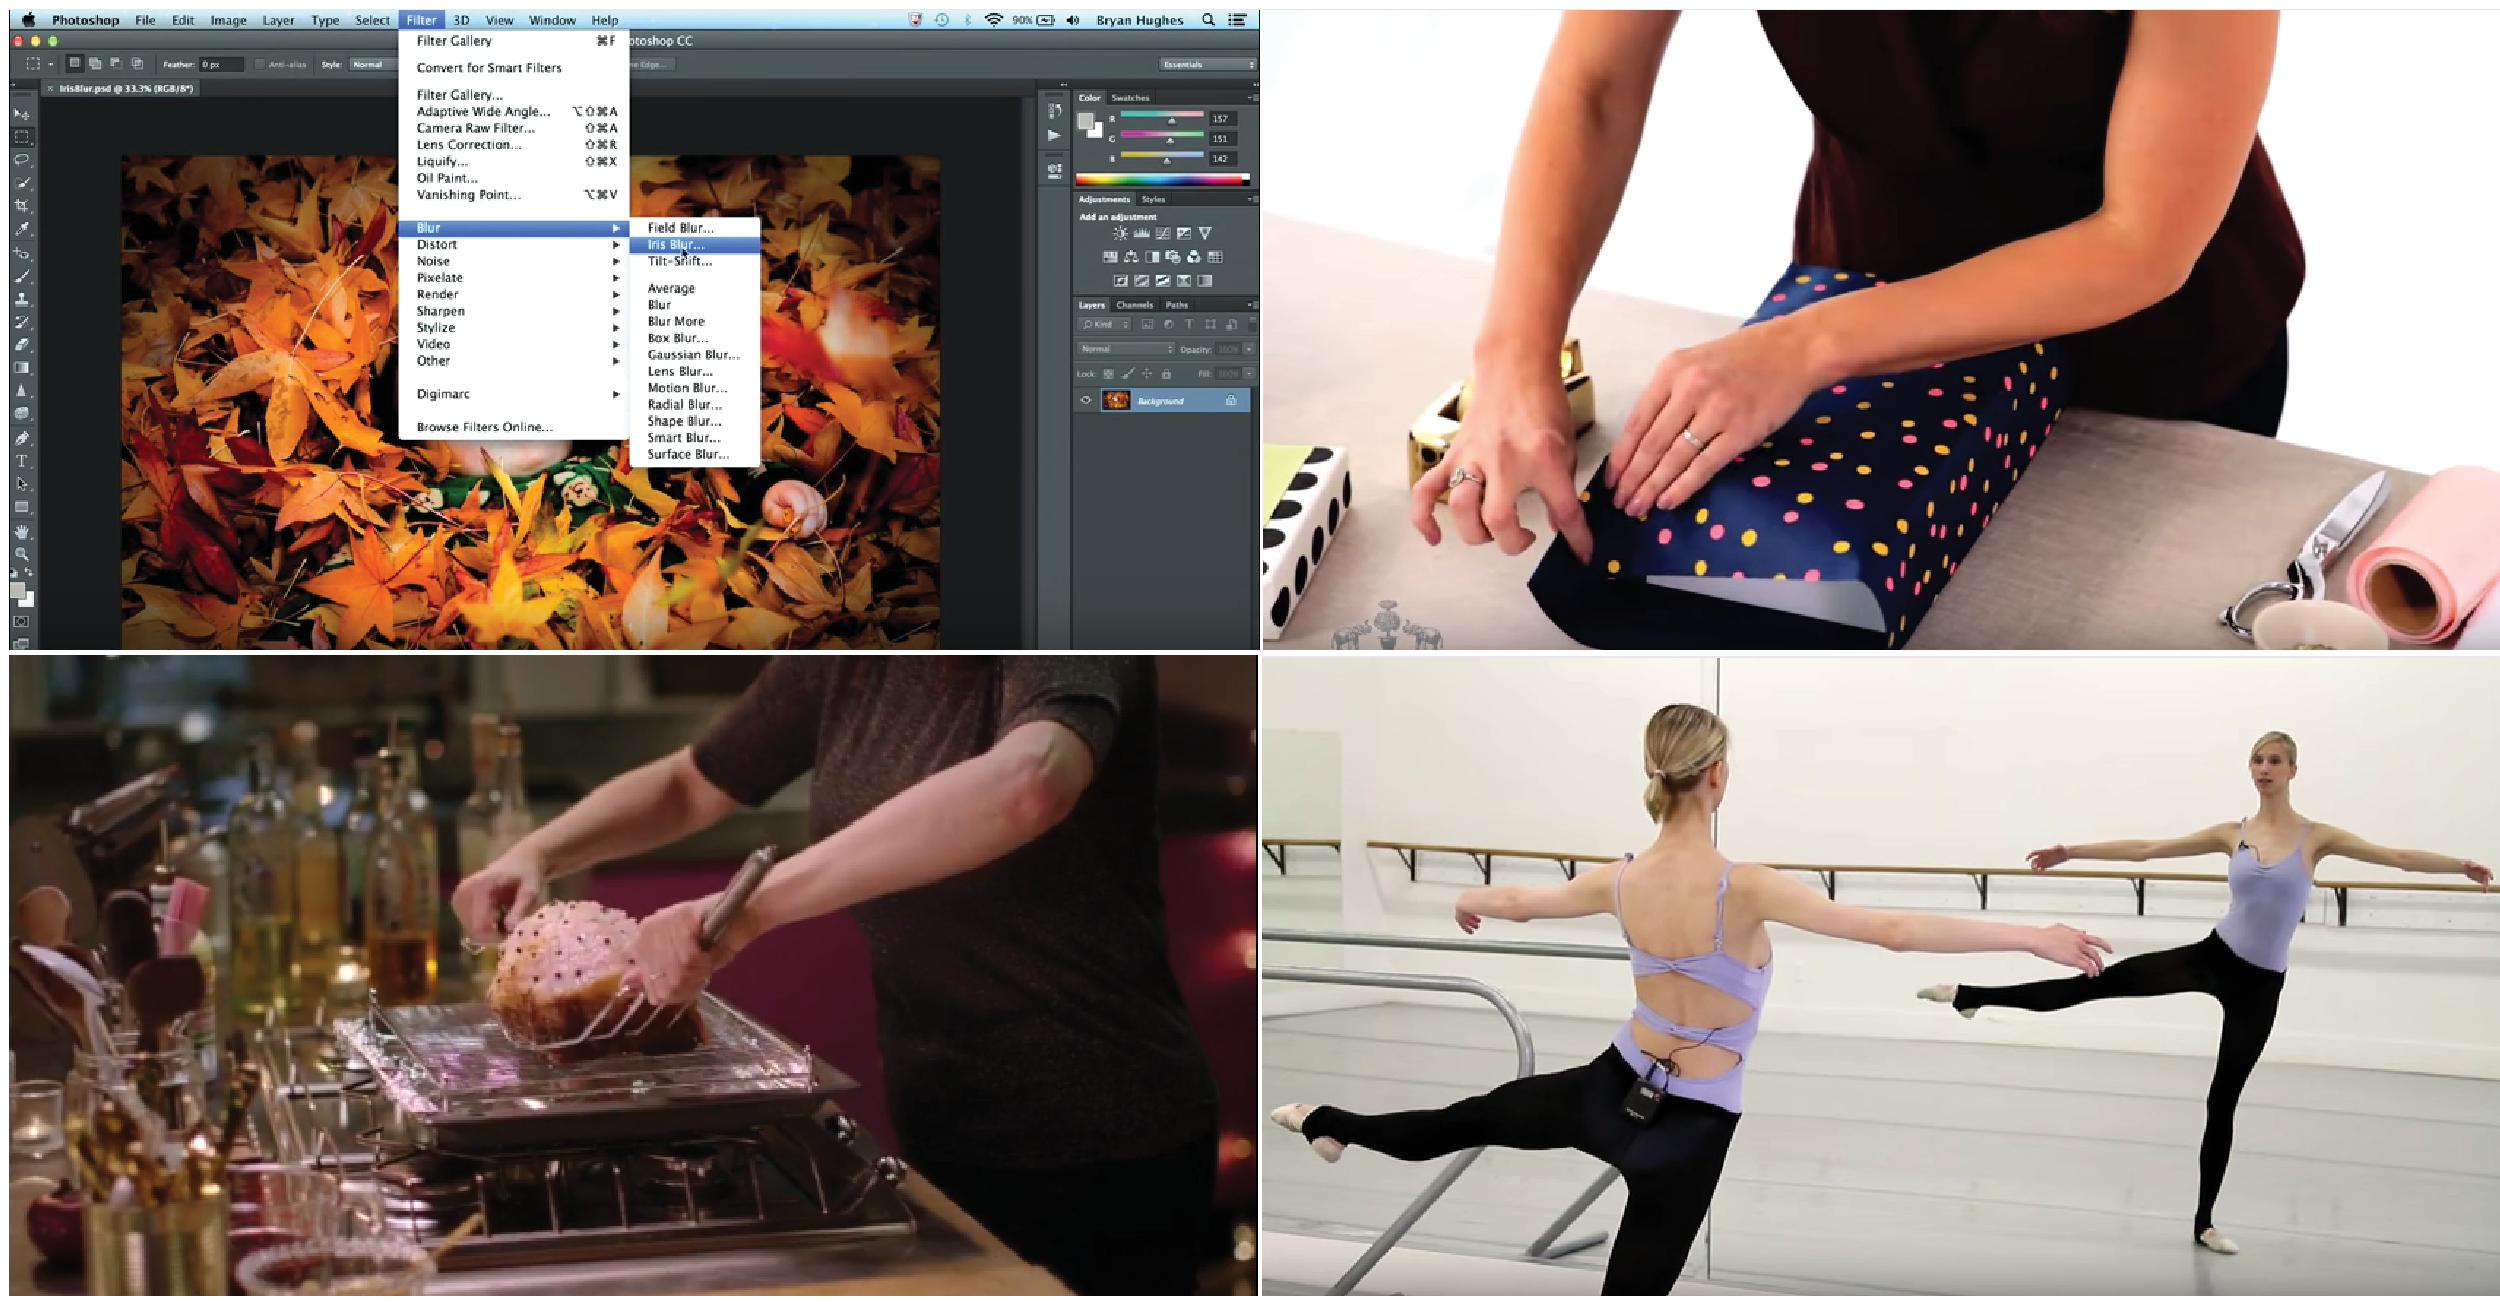
\includegraphics[width=\textwidth]{\background/fig/activities/activities}
  \caption[Example activities in tutorial domains.]{Example activities in tutorial domains:
  %
  a) image manipulations using a software application
  \footnote{``Photoshop Playbook: Selective Focus'', \url{https://youtu.be/Wh3ahxqDnyw} \copyright2016 with express permission from Adobe Systems Incorporated.},
  %
  b) wrapping a gift, a DIY task
  \footnote{``How to do a Japanese Gift Wrap'' by Rouge Shop, \url{https://youtu.be/Mf3IyeMF8ug}, licensed under CC BY 2.0},
  %
  c) cooking, an everyday activity
  \footnote{``How to Cook a Turkey in a Convection Oven'' by Six Sisters' Stuff, \url{https://youtu.be/QNkwKj1Vsuc}, licensed under CC BY 2.0}, and
  %
  d) golf lessons in sports
  \footnote{``Pat's Golf Tips Top of Swing Position'' by Blue Rock Golf Academy, \url{https://youtu.be/H06o7fMQSi4}, licensed under CC BY 2.0}.
  }
  \label{fig:background_activities}
  \end{minipage}
\end{figure*}

% A task-centric tutorial often involves domain-specific \keyword{know-how}, knowledge that is required to perform a task.
%
Instructional content is commonly structured as a list of \keyword{steps} or \keyword{subtasks} in a linear, \keyword{step-by-step} order.
%
It is important to include essential information required to complete a task, including materials, tools, preparation, expected outcome, and tips~\cite{Torrey:2007he}.
%
In some domains, instructions have developed into canonical domain-specific formats. For example, cooking recipes contain not only actions but also food ingredients and required amounts.
% The term \keyword{recipe} has been used for activities other than cooking.

Note that instructions are different from a (software) \keyword{documentation}, \keyword{manuals}, or \keyword{user guides}, which are technical documents contain non-task-centric details about a particular hardware or software system. A manual does not provide step-by-step guidance to follow. To accomplish a task, one needs to identify relevant information from the documentation and reason the workflow.

% -------------------

Instructions can be shown in different forms. There are two main forms of visual tutorials (see Figure~\ref{fig:background_formats}):
\begin{itemize}
  \item \keyword{Static tutorials}, which use text and figures to describe the set of operations required to accomplish a task. Such format is presented as a written document with a step-by-step list, while each step includes text description and/or an image or abstract illustration to describe the subtask. In some domains such as block or furniture assembly, a \keyword{diagram} or a pictorial summary shows the step procedure. Static tutorials are suitable for printing and are easy to scan because they show all instructions.
  \item \keyword{Video tutorials}, which are edited or raw videos of the tutorial author performing the task. Examples include screen recordings of a software application or a camera recording of a DIY task.
  %
  Video tutorials are composed of one or more ``shots,'' which is \iquote{the basic unit of an editor's film language, consisting of footage captured over a continuous duration of time without interruption}~\cite{Goldman:2007:FVA:1354647}, to provide the animation or capturing of movements in time.
  %
  They are effective to present the work in action, especially when the activities are hard to be described in text.
\end{itemize}

\begin{figure*}[th!]
  \centering
  \begin{minipage}{\textwidth}
  \includegraphics[width=\textwidth]{\background/fig/formats/formats}
  \caption[Major tutorial forms from online resources.]{
    Major tutorial forms from online resources \footnote{Combine photos on the go, \url{https://helpx.adobe.com/mobile-apps/how-to/combine-photos-photoshop-mix.html}} \footnote{Change the color of an object, \url{https://helpx.adobe.com/photoshop/how-to/change-color-object-photoshop.html}}:
    %
    a) Step-by-step static tutorials show a list of steps, each with text and figure(s) that describe a subtask, such as \iquote{Start combining photos} or \iquote{Refine your composite}, and
    %
    b) video tutorials show an author performing the task, which can be reviewed and controlled via a video player.
    \\
    \copyright2016 with express permission from Adobe Systems Incorporated.
  }
  \label{fig:background_formats}
  \end{minipage}
\end{figure*}

% -------------------

\subsection{Creating Instructions}
Instructions are created by one or more \keyword{authors} who document the process of completing a task and refine the material to a final deliverable.
%
Since the process often involves innovations and creations of the tasks of interests, authors can also be referred as \keyword{creators}, \keyword{makers}, or \keyword{hobbyists}.
%
Instructional authors are often the \keyword{professionals} or \keyword{experts} in the domains of their work. However, in tutorial production, they might be \keyword{amateurs} or \keyword{novices} who are not familiar with software tools to refine the documented material.

Throughout this dissertation, we call the process of author completing a task as a \keyword{demonstration} or a \keyword{performance}. Authors can therefore be as \keyword{demonstrators} or \keyword{presenters}.
%
In software, the demonstration process can be referred as a system \keyword{walkthrough}. Section \ref{background_creation} will discuss the production process of instructions.

% -------------------

\subsection{Consuming Instructions}
We define people who review instructional content as \keyword{viewers} or \keyword{learners}. Viewers may also be \keyword{followers} if they choose to follow the instructions in action to achieve the same or similar tasks.
%
Studies have shown that learners with different learning needs and habits have various preference on the tutorial formats. In Chapter \ref{chapter_mixt}, I'll examine these differences and propose a new instructional format.

% lecturer and online tutoring: involve more feedback collection and response to learners, beyond the scope of this paper

% -------------------------------------------

\section{Why Instructions?}
\label{background_why}

The research community has been investigating the motivations behind tutorial authors creating how-to videos and written instructions.
%
In early 90s, researchers studied users who formed online communities to collaboratively customize CAD systems \cite{Gantt:1992:GGP:142750.142767}. \iquote{Local experts} were found to play the key role within user groups. They provided supports to CAD system users of various levels of expertise by sharing customized environments and programmatic extensions. These experienced users were not professional programmers, but they were motivated by the frustrations of following manuals with existing software. They shared the materials in order to enhance manuals and help others acquire necessary skills.

The rise of maker movement from the 2000s introduced massive DIY project sharing via online services. Until mid-2016, Instructable has over 220,000 articles~\cite{InstructablesProjects}, and wikiHow provides 192,542 articles~\cite{wikiHowStatistics}.
%
Studies showed that one primary motivation of sharing DIY work is to demonstrate expertise ~\cite{Torrey:2007he,Kuznetsov:2010:REA:1868914.1868950}. Specifically, of the online survey that Kuznetsov and Paulos~\cite{Kuznetsov:2010:REA:1868914.1868950} conducted in 2010, 97\% of their 2608 respondents shared and contributed to projects to \iquote{Express myself/be creative.} Published tutorials serve as a way to broadcast skill and as an online portfolio.
%
Authors may derive revenue through advertising or referrals~\cite{Lafreniere:2012tl}, which was similar to how local, non-professional experts gained formal supports in CAD communities that Gantt \ea{}~\cite{Gantt:1992:GGP:142750.142767} found.

Viewers, on the other hand, typically seek technical explanations, but are also searching for inspiration~\cite{Torrey:2009fc} and looking for validation of existing skills~\cite{Lafreniere:2012tl}.
%
It was shown that people prefer web-based tutorials over manual as they provide \iquote{an immediate, specific goal to accomplish} and can help learners \iquote{shadow and experience an expert's work practices}~\cite{BenLafreniere:2013ux}.

While these studies present motivations beyond broadcasting and consuming instructions, research also found that creating ready-to-publish content can be time-consuming ~\cite{Kuznetsov:2010:REA:1868914.1868950}. Next, I discuss current techniques and practices of tutorial production.

% Make channel: 1,229,404 subscribers • 253,518,445 views
% Joined Mar 22, 2006
% https://www.youtube.com/user/makemagazine
% June 19, 2016
% \cite{MakerMediaKit}

% -------------------------------------------

\section{Techniques of Effective Instructions}
\label{background_techniques}

Following instructions can be an intense process for a learner, especially when performing unfamiliar, complicated tasks. Therefore, tutorial authors have to carefully provide concise, effective instructions that can be interpreted by a follower efficiently. A set of techniques has been developed and widely used in technical and everyday instructions.

length~\cite{Black:1986:KMI:29933.275623}

% -------------------

\subsection{Visual Annotations}
% \label{background_techniques_visual}

\begin{table*}[!htbp]
  \centering
  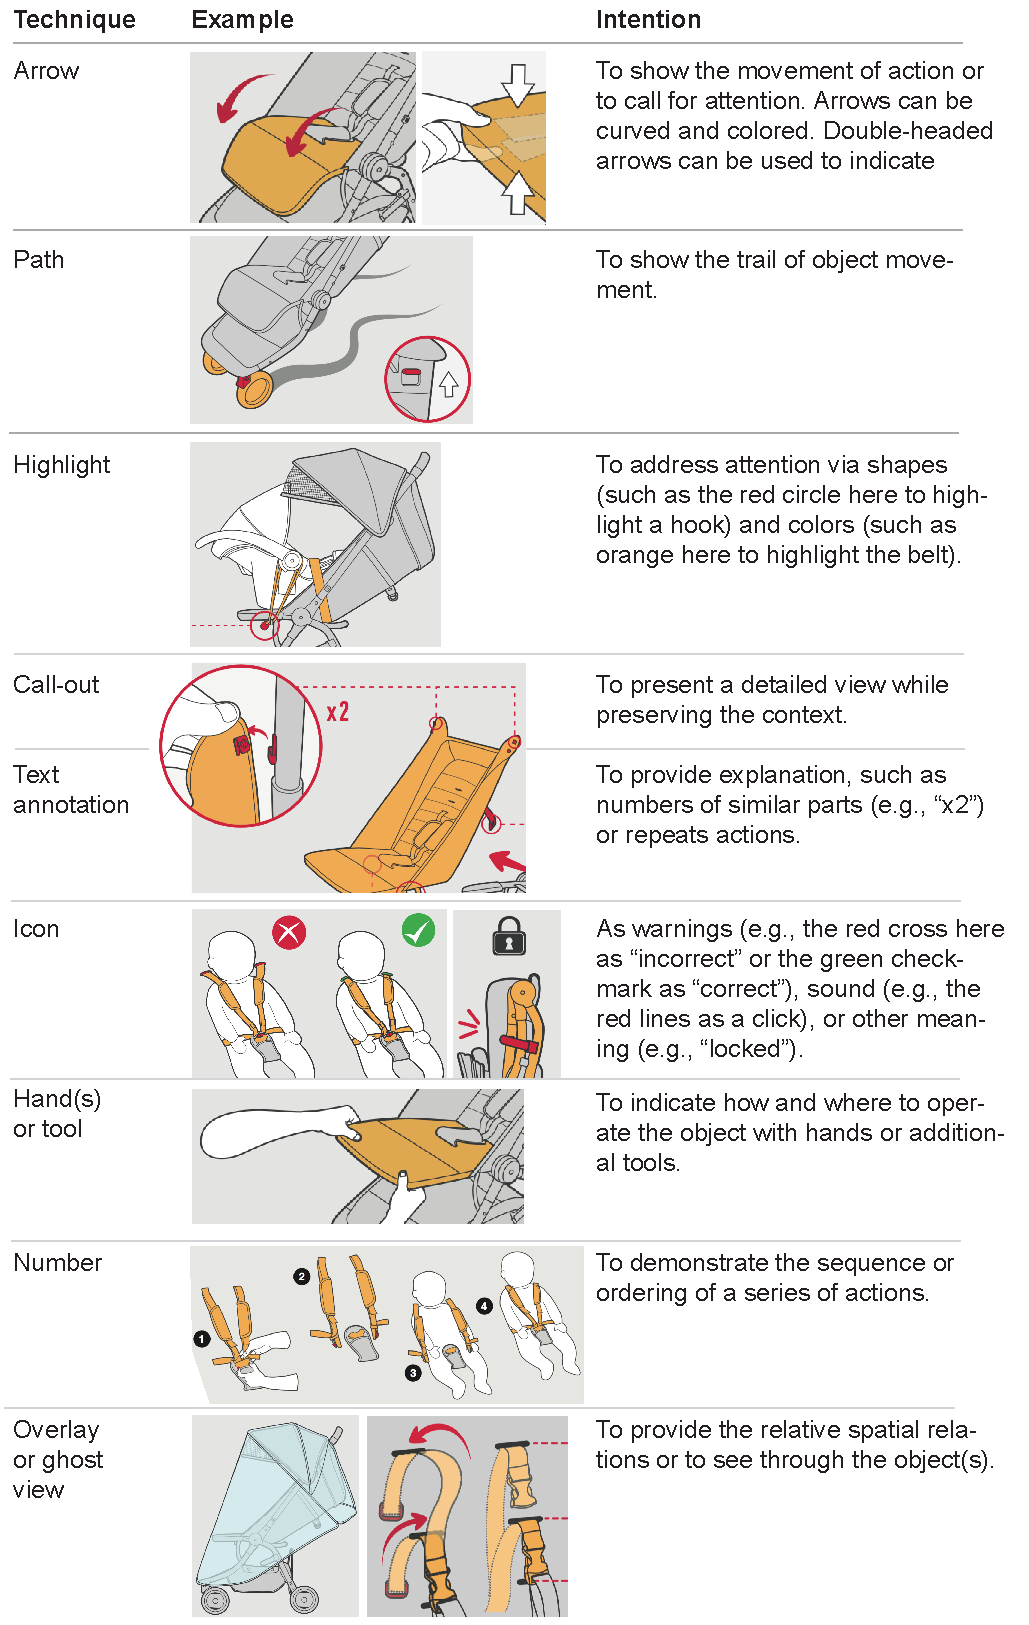
\includegraphics[width=0.78\columnwidth]{\background/fig/techniques/techniques}
  \caption{A list of annotation techniques that are often used to provide instructions. Examples are selected from stroller instructions~\cite{MountainBuggyInstructions}. Reproduced with permission.}
  \label{background_annotation_techniques}
\end{table*}
% https://support.mountainbuggy.com/hc/en-us/articles/203682124-List-of-product-instructions

To help learners quickly identify key information, visual annotations are commonly used. Table~\ref{background_annotation_techniques} shows a list of annotation techniques in practices that I summarized from book material for static tutorials~\cite{mijksenaar1999open,greenberg2012sketching,Buxton:2007:SUE:1526229,tufte1990envisioning}, but some of these techniques are often applied in video tutorials (see Table~\ref{background_video_annotation_techniques}).
%
These visual elements are effective to indicate the movement of action or objects (via arrows or paths), identify important parts (via highlights), present the details and overview (via call-outs), and provide additional messages such as a warning (via icons or text).

To present annotations, Tufte~\cite{tufte1990envisioning} described the importance of layering information: \iquote{Among the most powerful devices for reducing noise and enriching the content of displays is the technique of layering and separation, visually stratifying various aspects of the data.}
%
Color, for example, is effective to separate content. Shown in Table~\ref{background_annotation_techniques}, motion arrows are presented in red, paths are in a darker gray color, and the key components are highlighted in orange or white. The design goal is to help learners efficiently capture important actions and tips.
%
Figure~\ref{fig:background_HubbleExploded} shows another example of using colors to separate abstract information. In this exploded diagram of the Hubble Space Telescope, the labels or text annotations are in black, with blue lines pointed to individual parts, that differentiate from the machine components presented in green.

\begin{figure*}[th!]
  \centering
  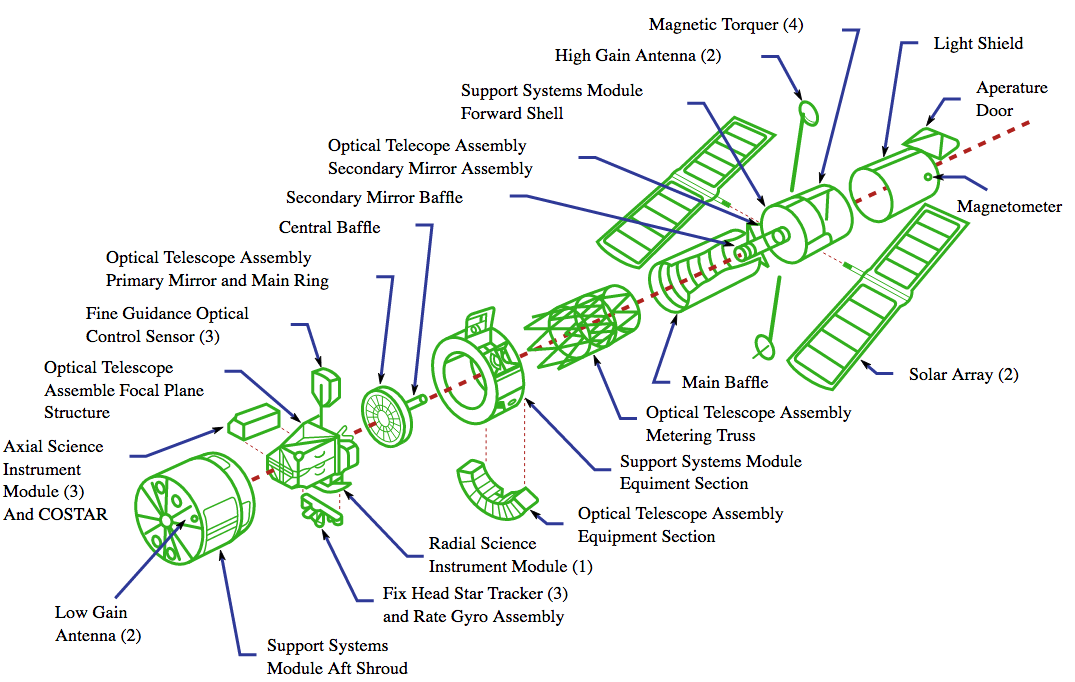
\includegraphics[width=0.8\textwidth]{\background/fig/layering/HubbleExploded}
  \caption{Color can differentiate between annotation (labels in black) and annotated information (parts in green in this diagram). Image by AndrewBuck (Own work), licensed under CC BY-SA 3.0.
  }
  \label{fig:background_HubbleExploded}
\end{figure*}

% https://www.ifixit.com/Guide/LG+G+Watch+R+Motherboard+Replacement/50124#undefined

% \clearpage

% \begin{table*}[h!]
%   \centering
%   \begin{minipage}{\textwidth}
%   \includegraphics[width=\textwidth]{\background/fig/video_techniques/video_techniques}
%   \caption[Example editing techniques applied to video tutorials to provide concise instructions.]{Example editing techniques applied to video tutorials selected from two instructional videos produced by the same company (a and c left from
%   \footnote{Mountain Buggy, Nano™ Instructional Guide, \url{https://youtu.be/p6MzLXeWBJw}} and others from
%   \footnote{Mountain Buggy, Urban Jungle ™ Stroller Instructions, \url{https://youtu.be/QwCtdpDmYu8}}):
%   a shows a vignette effect on a shot; b first shows an overview shot, and then jumps to a close-up; c presents a title page (left) and text annotation (right); d shows animation of illustrations.
%   }
%   \label{fig:background_techniques_to_videos}
%   \end{minipage}
% \end{table*}

% -------------------

\subsection{Static Diagrams}

Static, step-by-step instructions are composed of one or more figures, which can be either illustrations, images, or software screenshots. One form is to list steps in a document with a sequence of numbered steps (see Figure~\ref{fig:background_formats}a). Images are carefully chosen...
%
A series of actions can also be presented in one combined diagram with a clear layout. \tofix{add more info}

% Information should be visually concise and distinguishable.
% More advanced techniques such as overlaying visual components or composing an exploded view can be useful to show the depth of spatial relations between detailed components.

% Tufte pointed out that the top design does not effectively separate the information, including an actor (in silhouette), a prop (the light with lamp-whiskers), actions (the directional arrows), the text descriptions, and the grid boxes of individual diagrams. The visuals are ``too loud and too similar'' as all the elements are in black and the weights are equally heavy among boxes, arrows, and text.
% The revised design, shown at the bottom of the figure, separates elements from the actor: the glowing light is colored in yellow and whiskers are removed (not to confused with trembling motion); motion arrows are highlighted in red; the weight of the grid border is lighted to avoid confusion with motion arrows; silhouette is shown in gray to bring more emphasis on other information; text is shown with a lighter font.

% \begin{figure*}[th!]
%   \centering
%   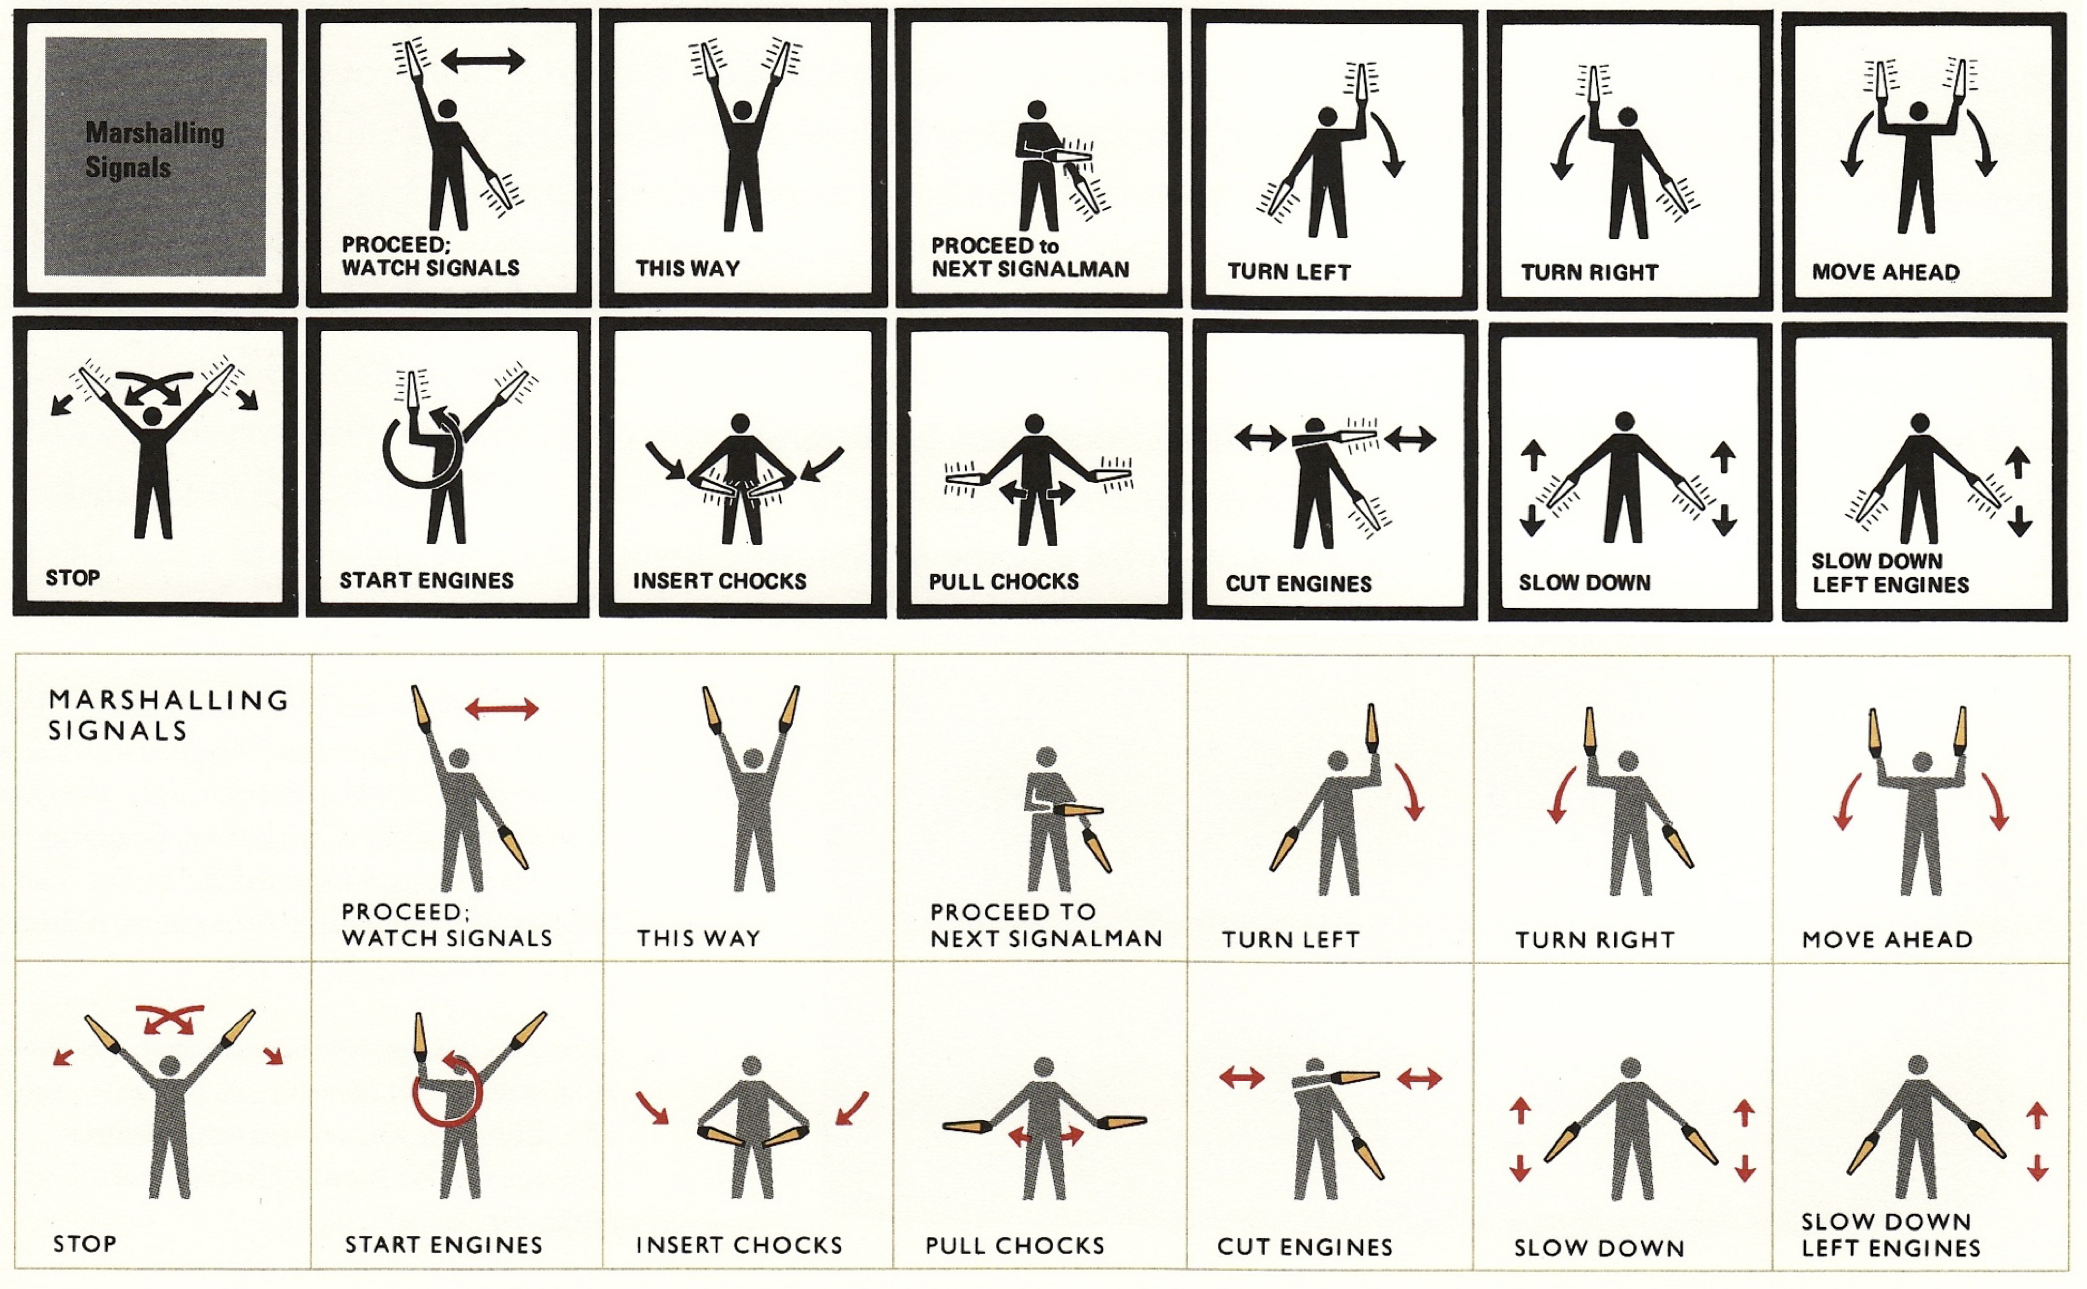
\includegraphics[width=\textwidth]{\background/fig/layering/Tufte_layeringp63}
%   \caption{By carefully designing visual elements using color and weight, information can be visually separated~\cite{tufte1990envisioning}. The bottom design is revised from the top example via changes of these factors.
%   }
%   \label{fig:background_marshalling}
% \end{figure*}

% Automated Generation of Interactive 3D Exploded View Diagrams

% -------------------

\subsection{Video Editing Techniques}

\begin{table*}[!htbp]
  \centering
  \includegraphics[width=\textwidth]{\background/fig/video_techniques/video_techniques_annotation}
  \begin{minipage}{\textwidth}
  \caption[Example annotation techniques used in a video tutorial.]{
    Example annotation techniques used in a video tutorial\footnote{``How to use Loola 3 stroller'' by Maxi-Cosi, \url{https://youtu.be/p6MzLXeWBJw}, licensed under CC BY 2.0}.
  }
  \label{background_video_annotation_techniques}
  \end{minipage}
\end{table*}

In addition to enhancing a shot with visual annotations, several conventional video editing techniques are often seen. A \textbf{close-up} is useful to zoom in a shot to demonstration a detailed view. Figure~\ref{fig:background_video_techniques}a shows one example that the video switches from an overview (to provide context of the position), to a detailed view (to show how exactly the action should be performed), back to an overview (to walk to the other side), and again to a detailed view.

Static tutorials present several steps in a document that can be quickly glanced by a learner to get an overview. On the contrary, as video tutorials present instructions continuously, it is important to help viewers keep track of important steps. \textbf{Title scenes} are one common technique to provide a distinct change for a new section (see Figure~\ref{fig:background_video_techniques}b).

\begin{figure*}[h!]
  \centering
  \includegraphics[width=\textwidth]{\background/fig/video_techniques/video_techniques}
  \begin{minipage}{\textwidth}
  \caption[Example video editing techniques used in a video tutorial.]{
    Example video editing techniques used in a video tutorial\footnote{``How to use Loola 3 stroller'' by Maxi-Cosi, \url{https://youtu.be/p6MzLXeWBJw}, licensed under CC BY 2.0}:
    %
    (a) a sequence of overview and detailed shots, and
    (b) a title scene to introduce a new section, which can include animation or movement as a preview.
  }
  \label{fig:background_video_techniques}
  \end{minipage}
\end{figure*}

% -----------

When providing instructions, \emph{operation time} is an important factor to guide learners through a task in order to provide awareness of how much time one should allocate.
%
However, to provide concise information, time is often manipulated by two ways: 1) applying a \textbf{fast-forward} or \textbf{slowdown} effect to a shot, or 2) jumping (a ``cut'') between two consecutive shots, often with a visual \textbf{transition} effect, such as fades, dissolves, or wipes. These techniques are commonly used to condense long or repetitive actions in raw footage. The latter is especially common when partial footage is removed, such as mistakes or long breaks~\cite{Tseng:2014:PVP:2598510.2598540}.
%
When these effects are applied, it is important to clearly convey the time manipulation to a viewer. Subtitles, text annotation, or narration can provide such indication, e.g., ``5 minutes later'' or ``x10'' (which means 10 times faster than the original playback speed).

% \textbf{Auditory effects} can guide learners .

% https://youtu.be/Wv7sdHEdaR0?t=1m41s
% Concise video tutorials commonly include annotation techniques, including applying arrows, paths, highlights, call-outs, and text~\cite{Chi:2013:DGC:2501988.2502052} (see Figure~\ref{fig:background_video_techniques}a). Vignette or dark edges are rare but could be used to highlight a video subview (see Figure~\ref{fig:background_video_techniques}a).

% -----------

Online video tutorials are commonly found to be 2-10 minutes long~\cite{Chi:2013:DGC:2501988.2502052}. Our formative study with 6 YouTube authors showed that this strategy is to provide enough information for viewers to understand the demonstration, but at the same time keep the video lively and interesting. This editing goal is applied to online videos when viewers tend to have shorter attention spans~\cite{YouTubeVideoLength2016,YouTubeVideoLength2012}, not for conventional industrial video production.

As videos contain a series of steps and details, common video players, however, only support a timeline for navigation. Viewers can jump to a certain point of a video with the timeline, or adjust the playback speed, but the mapping between time and steps is missing. It can also be difficult to glance through the video and reason the complexity in each step.
%
To fill in the gap between a video and a list of steps or topics, some tutorial authors choose to provide additional text description listing the \textbf{index} to the video. Figure~\ref{fig:background_video_index} shows an example from a YouTube video. A list of 12 items and their starting time in the video are included in the video description, which is placed below the video player. The YouTube web interface automatically adds links to the timestamps shown as blue links. By following these links, viewers can skip to a specific topic.

show face~\cite{Kizilcec:2014:SFV:2556288.2557207}

\begin{figure*}[h!]
  \centering
  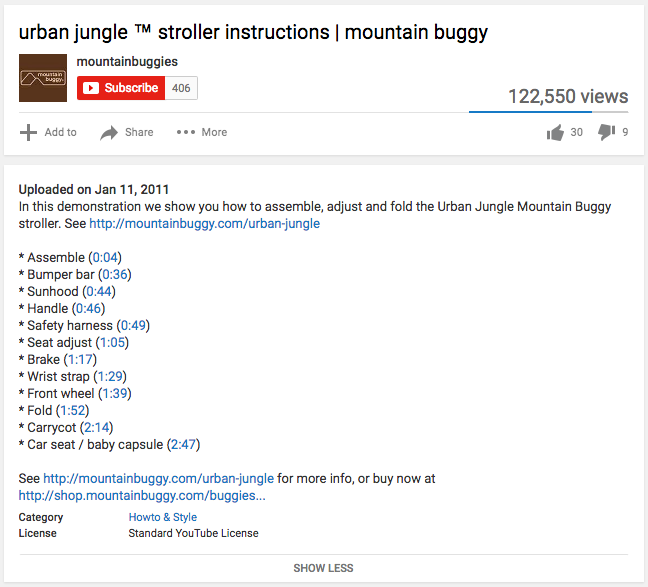
\includegraphics[width=0.7\textwidth]{\background/fig/video_index/index_highlighted}
  \begin{minipage}{\textwidth}
  \caption[Example video index to video instructions provided by authors for viewers to navigate between topics.]{
    Example video index to video instructions\footnote{Mountain Buggy, Urban Jungle ™ Stroller Instructions, \url{https://youtu.be/QwCtdpDmYu8}} provided by authors for viewers to navigate between topics.
  }
  \label{fig:background_video_index}
  \end{minipage}
\end{figure*}

% \vspace{12pt}
% \fbox{
%   \centering
% \begin{minipage}{25em}
%   In this demonstration we show you how to assemble, adjust and fold the Urban Jungle Mountain Buggy stroller. See http://mountainbuggy.com/urban-jungle

%   * Assemble (0:04)

%   * Bumper bar (0:36)

%   * Sunhood (0:44)

%   * Handle (0:46)

%   * Safety harness (0:49)

%   * Seat adjust (1:05)

%   * Brake (1:17)

%   * Wrist strap (1:29)

%   * Front wheel (1:39)

%   * Fold (1:52)

%   * Carrycot (2:14)

%   * Car seat / baby capsule (2:47)
% \end{minipage}
% }

% -------------------------------------------

\section{Instruction Production Process}
\label{background_creation}

\begin{quote}
\iquote{The practice of writing and sharing DIY tutorials is at the heart of the distributed production and creativity of DIY. Tutorials not only provide tutorship of particular projects, they also develop the skills and competences of those involved in DIY and, in doing so, expand the culture and practices of DIY. It is fair to say that the vitality of DIY practices relies on the effectiveness and quality of tutorials.} -- Wakkary \ea{}~\cite{Wakkary:2015:TAH:2702123.2702550}
\end{quote}

In their paper discussing tutorial authorship, Wakkary \ea{}~\cite{Wakkary:2015:TAH:2702123.2702550} pointed out the values of producing DIY tutorials, which I believe can be applied to instructions of other domains. However, the time required to create a tutorial is the primary concern for authors~\cite{Kuznetsov:2010:REA:1868914.1868950,Tseng:2014:PVP:2598510.2598540}, especially for activities that involve multiple steps, tools, and materials. To produce a tutorial, an author may go through several stages:
% Key findings include identifying tools and components and structuring a task into steps with a clear sequence.

Torrey \ea{}~\cite{Torrey:2007he} proposed a project lifecycle of three phases. First, the ``project'' involves a goal or a challenge to achieve. Second, the ``story'' documents the making via words and text. Third, the ``contribution'' broadcasts the How-To.
%
Similarly, Tseng and Resnick~\cite{Tseng:2014:PVP:2598510.2598540} found that ``documenting'' and ``designing'' a DIY project for documentation are often separate processes.
%
Our interviews with instructional authors on YouTube suggested that a production process can be similar to a filming production~\cite{Chi:2013:DGC:2501988.2502052}.
%
In sum, Figure~\ref{fig:background_creation} shows a typical tutorial creation workflow that we identified, which includes four main stages: \iquote{planning} a procedure of achieving the goal of a task or a project, \iquote{recording} the process of completing the project, \iquote{editing} the captured material into a form that can be followed, and finally \iquote{sharing} the instructions to the communities.
%
Some tutorial creators, especially professionals, may work as a team with multiple role players in a production process, while some work individually. The time required to create a tutorial may vary from a few minutes to weeks.

Below I describe the characteristics of each stage in detail.

\begin{figure*}[h!]
  \centering
  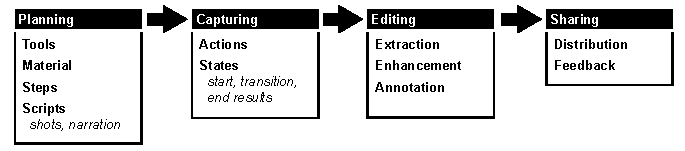
\includegraphics[width=\textwidth]{\background/fig/creation_process}
  \caption{A common workflow of tutorial creation, which includes planning the task in detail, recording the process, editing the captured content into a readable form, and sharing with the communities.}
  \label{fig:background_creation}
\end{figure*}

% ------------------------

\subsection{Planning}
Planning or preparation helps authors gather ideas, inspirations, and necessary details prior to building a tutorial project~\cite{Torrey:2007he}. At this stage, authors decide the project scope and expected outcome, confirm the material and tools required, and design subtasks or steps to be executed. Some authors choose to explicitly write detailed scripts to explain their activities during the recording stage~\cite{Chi:2013:DGC:2501988.2502052}. Figure~\ref{fig:background_scripts} presents examples of instructional video scripts.

\begin{figure*}[th!]
  \centering
  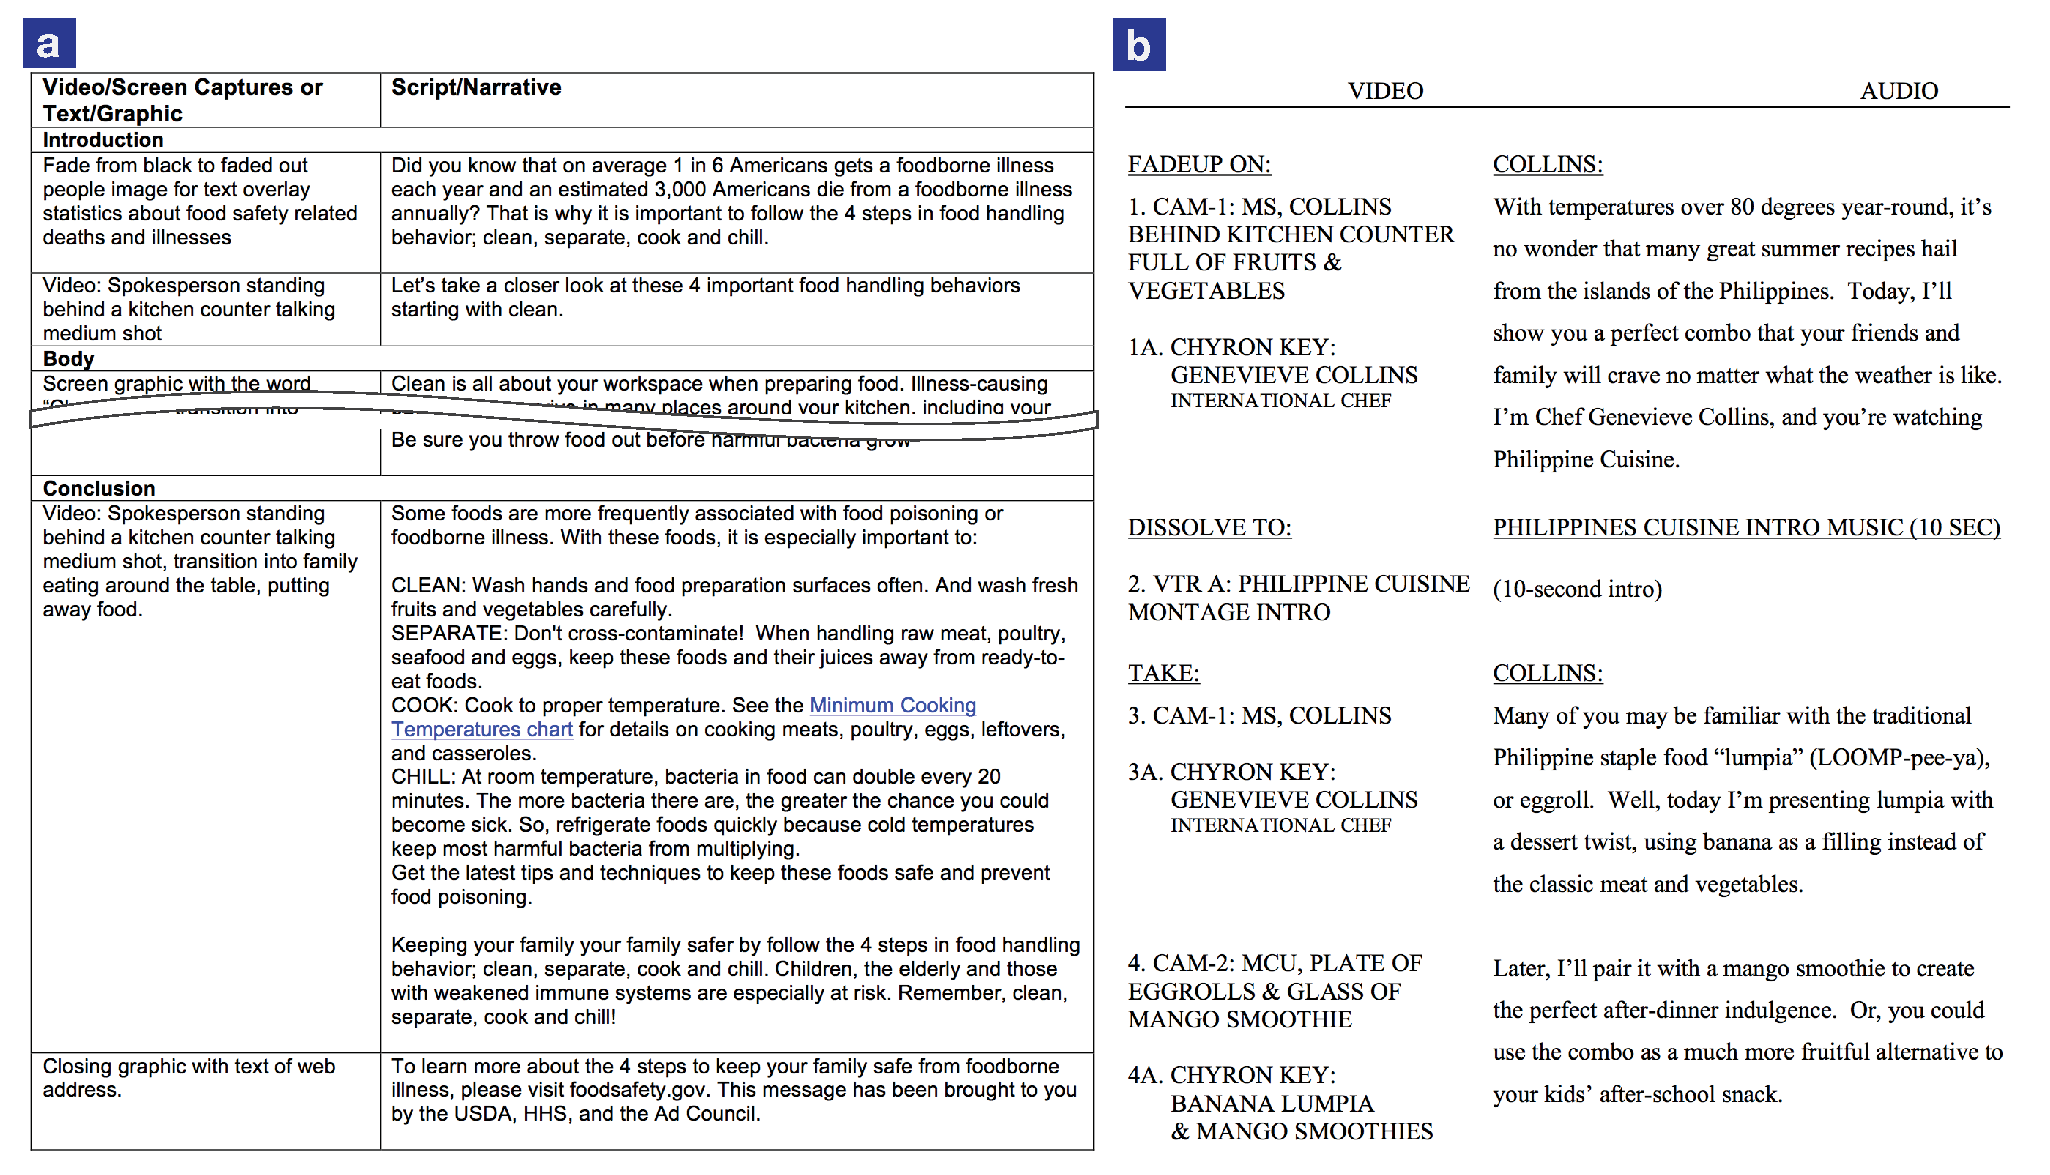
\includegraphics[width=\textwidth]{\background/fig/scripts/scripts}
  \caption{Example scripts for instructional videos about a) food safety~\protect\cite{WisconsinFoodSafetyScript} and b) cooking ~\protect\cite{SouthernIllinoisScript}. Each includes video shot(s) and narration, some with additional notes on the actions. High-level structure can also be specified, such as ``introduction'' and ``conclusion.''}
  \label{fig:background_scripts}
\end{figure*}

\subsection{Recording}
% TODO: One question as I read this: Do authors perform only once? In many other media production pipelines, this is an iterative process - write a draft, then improve it; record a shot, critique it, maybe re-record if necessary.
Documenting or recording is the core of creating instructions in order to guide viewers through a specific task. At this stage, authors document the process of a task demonstration via recording devices, such as digital cameras, camcorders, and mobile devices. They capture necessary actions using tools and materials, as well as the changing of states of the elements.
%
Multimedia material has been found to be effective to document procedural knowledge~\cite{Kuznetsov:2010:REA:1868914.1868950,Wakkary:2015:TAH:2702123.2702550}, including:

\begin{itemize}
  \item Static photographs that capture specific moments in a procedure.
  \item Video footages that record a computer screencast or a scene of a demonstration.
  \item Audio recordings that preserve the sound of activities or author narration. The narration can be transcribed into text for reading.
  \item Other domain-specific content (e.g., code, circuit board layouts, 3D models, and sketches) or resources (e.g., books or URLs to other material), which often serve as supplementary material.
\end{itemize}

\subsection{Editing}
After collecting necessary material, the majority of efforts and time often devotes to editing--to turn the raw material to a concise form.
Photographs need to be cropped and resized~\cite{Tseng:2014:PVP:2598510.2598540}, sometimes annotated~\cite{Torrey:2007he}; videos require removing footage, applying visual effects and transitions; audio has to be processed to omit utterances and condense narration~\cite{Chi:2013:DGC:2501988.2502052}. Popular editing tools include Adobe Photoshop and Apple Final Cut Pro, and emerging mobile applications such as Snapguide have been adopted by novices.

Different multimedia forms can be mixed to create tutorial formats mentioned in Section~\ref{background_terms}. Videos, in particular, have become a popular medium to document and demonstrate the functionality of the work:

\begin{quote}
\iquote{Videos, for instance, require a long time to edit, but can influence the viewer in at least three powerful ways: 1) by physically illustrating the steps required to create an artifact; 2) by showcasing a new idea in its functional form; and 3) by directly `speaking' to and engaging with the audience.} -- Kuznetsov and Paulos~\cite{Kuznetsov:2010:REA:1868914.1868950}
\end{quote}

\subsection{Sharing}
Finally, authors may release the refined content and share the deliverable with others. Common media or platforms include: personal blogs, content sharing sites, forums, emails, or personal networks.
%
Some of these channels offer ways for the audience to provide feedback and contribute. Lafreniere \ea{}~\cite{Lafreniere:2012tl} specifically analyzed the online comments to web tutorials. Their study shows that the audience has several purposes to communicate via comments, including technical validation and refinement, which can be useful for authors to improve their documentation techniques.

% , depending on the stages involved and the content.

% -------------------------------------------

\section{Summary}

These studies and observations suggest that tutorials have a larger variety of purposes and uses than merely communicating technical content.
%
In my dissertation, I strive to make authoring of instructions more accessible to amateurs while maintaining opportunities for adding individual style through control over editing effects.
%
Next, I survey prior work on computational methods of supporting authoring and following instructions.
